\chapter{Modelarea jocului}

\section{Bazele jocului Monopoly}
\subsection{Elementele jocului}
Jocul Monopoly se bazează pe concurența jucătorilor cu scopul stabilirii unui monopol capitalist în speranța obținerii unui venit pasiv stabil și profitabil. Acesta se bazează pe elemente stocastice precum aruncarea zarurilor și cartonașele „Cufărul Comunității" și a celor „Șansa" pentru a încerca să uniformizeze cât mai mult șansa de câștig.

Monopoly dispune de o tablă divizată în 40 de căsuțe, subdivizate în 5 categorii, pe baza rolului acestora în joc. De asemenea acesta mai beneficiază și de elemente adiacente ce contribuie la complexitatea și deciziile luate:

\begin{itemize}
    \item \textbf{Proprietățile imobiliare}: Sunt zonele cumpărabile ce simbolizează un cartier, zonă sau bulevard din lumea reală, grupate după o culoare ce reprezintă aprecierea acestora. Jucătorii se întrecu în cumpărarea acestora, urmând ca apoi orice alt jucător ce nu deține proprietatea să fie considerat un chiriaș, fiind nevoit să plătească chirie proprietarului.
    \item \textbf{Case și hoteluri}: Sunt modalități de îmbunătățire a venitului pasiv și consolidării monopolului deținut. Odată deținute toate proprietățile de aceeași culoare, se consideră că jucătorul deține monopol pe culoarea respectivă, acesta putând amplasa case și hoteluri cu scopul măririi chiriei percepute pe fiecare proprietate.
    \item \textbf{Gările}: Sunt zone cumpărabile, ce se diferențiază prin caracterul lor static (nu pot fi îmbunătățite), dar care contribuie prin incrementarea chiriei percepute pe fiecare unitate, prin numărul lor.
    \item \textbf{Utilitățile}: Sunt zone cumpărabile, statice, ce beneficiază de mărirea chiriei pe baza unui factor de multiplicare în urma aruncării zarurilor. Ca și în cazul gărilor, numărul utilităților deținute, îmbunătățește considerabil chiria percepută.
    \item \textbf{Șansa și Cufărul Comunității}: Sunt căsuțe ce necesită extragerea unui cartonaș din teancul corespunzător și executarea acțiunii imediat al acestuia.
    \item \textbf{Cartonașele Șansa și Cufărul Comunității}: Acestea ascund atât evenimente negative, precum plătirea unui impozit, cât și evenimente neutre sau ajutătoare.
    \item \textbf{Căsuțele Taxă}: Sunt căsuțe ce necesită plata imediată a unei sume afișate.
    \item \textbf{Căsuțele din colțuri}: Sunt elemente definitorii pentru joc, ele având diferite acțiuni.
    \item \textbf{Banii}: Sunt resursele cu care jucătorii interacționează cu mediul, folosindu-i pentru a cumpăra sau finaliza acțiuni.
\end{itemize}

\begin{figure}[H]
    \centering
    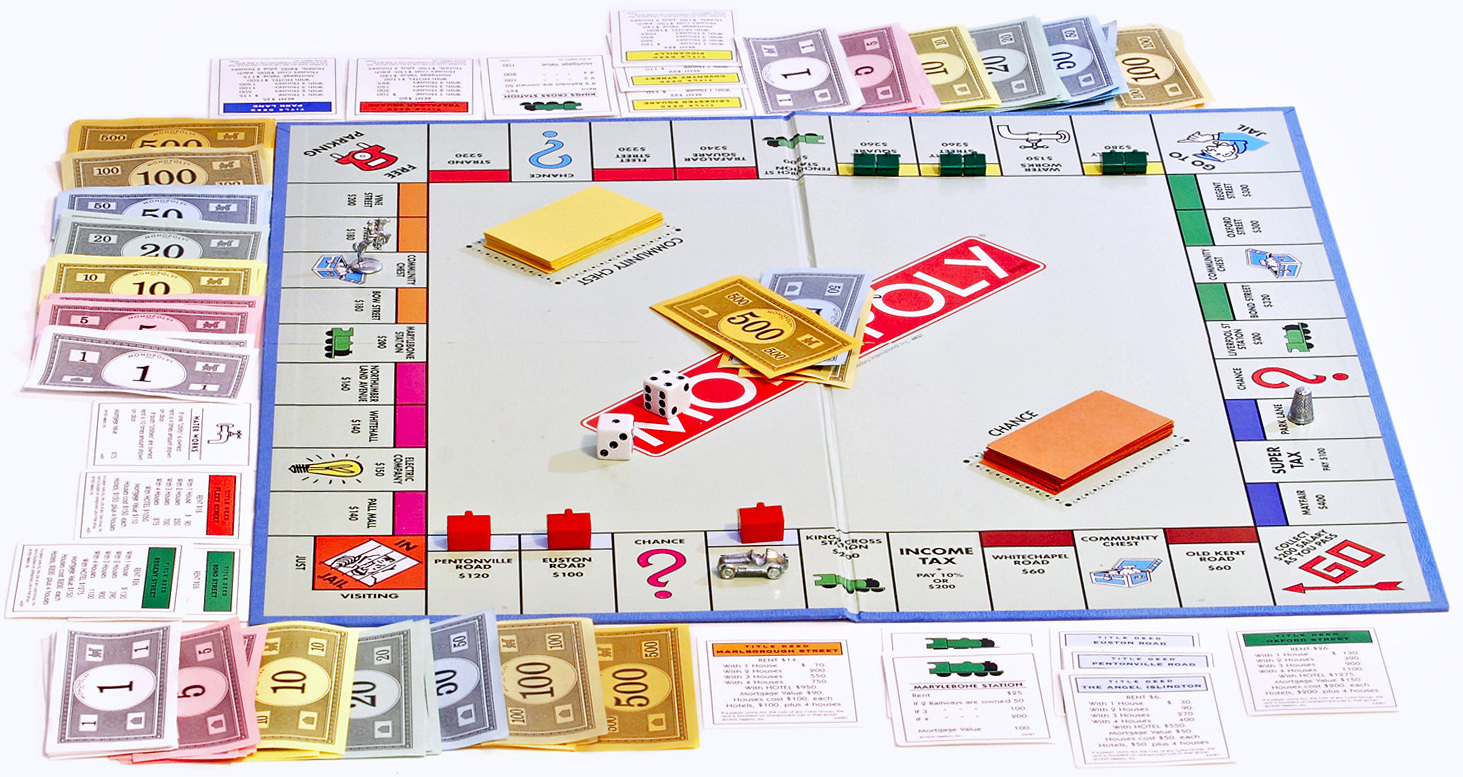
\includegraphics[width=10cm]{images/monopoly_elements.jpg}
    \caption{Elementele disponibile în jocul Monopoly \cite{wikipedia_monopoly}}
    \label{fig:monopoly-elements}
\end{figure}

\subsection{Regulile jocului}
Conform regulilor oficiale \cite{monopoly_rules}, jocul este conceput pentru a fi jucat de 2-4 jucători. Fiecare jucător dispune de un pion și primește o sumă inițială de 1500₩ (simbolul specific al banilor monopoly \cite{monopoly_money}). Jucătorul cel mai tânăr își începe aruncarea zarurilor după își continuă acțiuniile în funcție de căsuța în care a ajuns, rândul său încheindu-se și fiind pasat următorului jucător ca vârstă. Printre acțiunile posibile amintim de: cumpărarea unei proprietăți, licitație pentru o proprietate, cumpărarea unei case, etc. Ordinea definirii acțiunilor și posibilitatea executării lor sunt redate într-o formă sumară în diagrama stărilor din joc \ref{fig:monopoly-rules-state-machine}.

\begin{figure}[H]
    \centering
    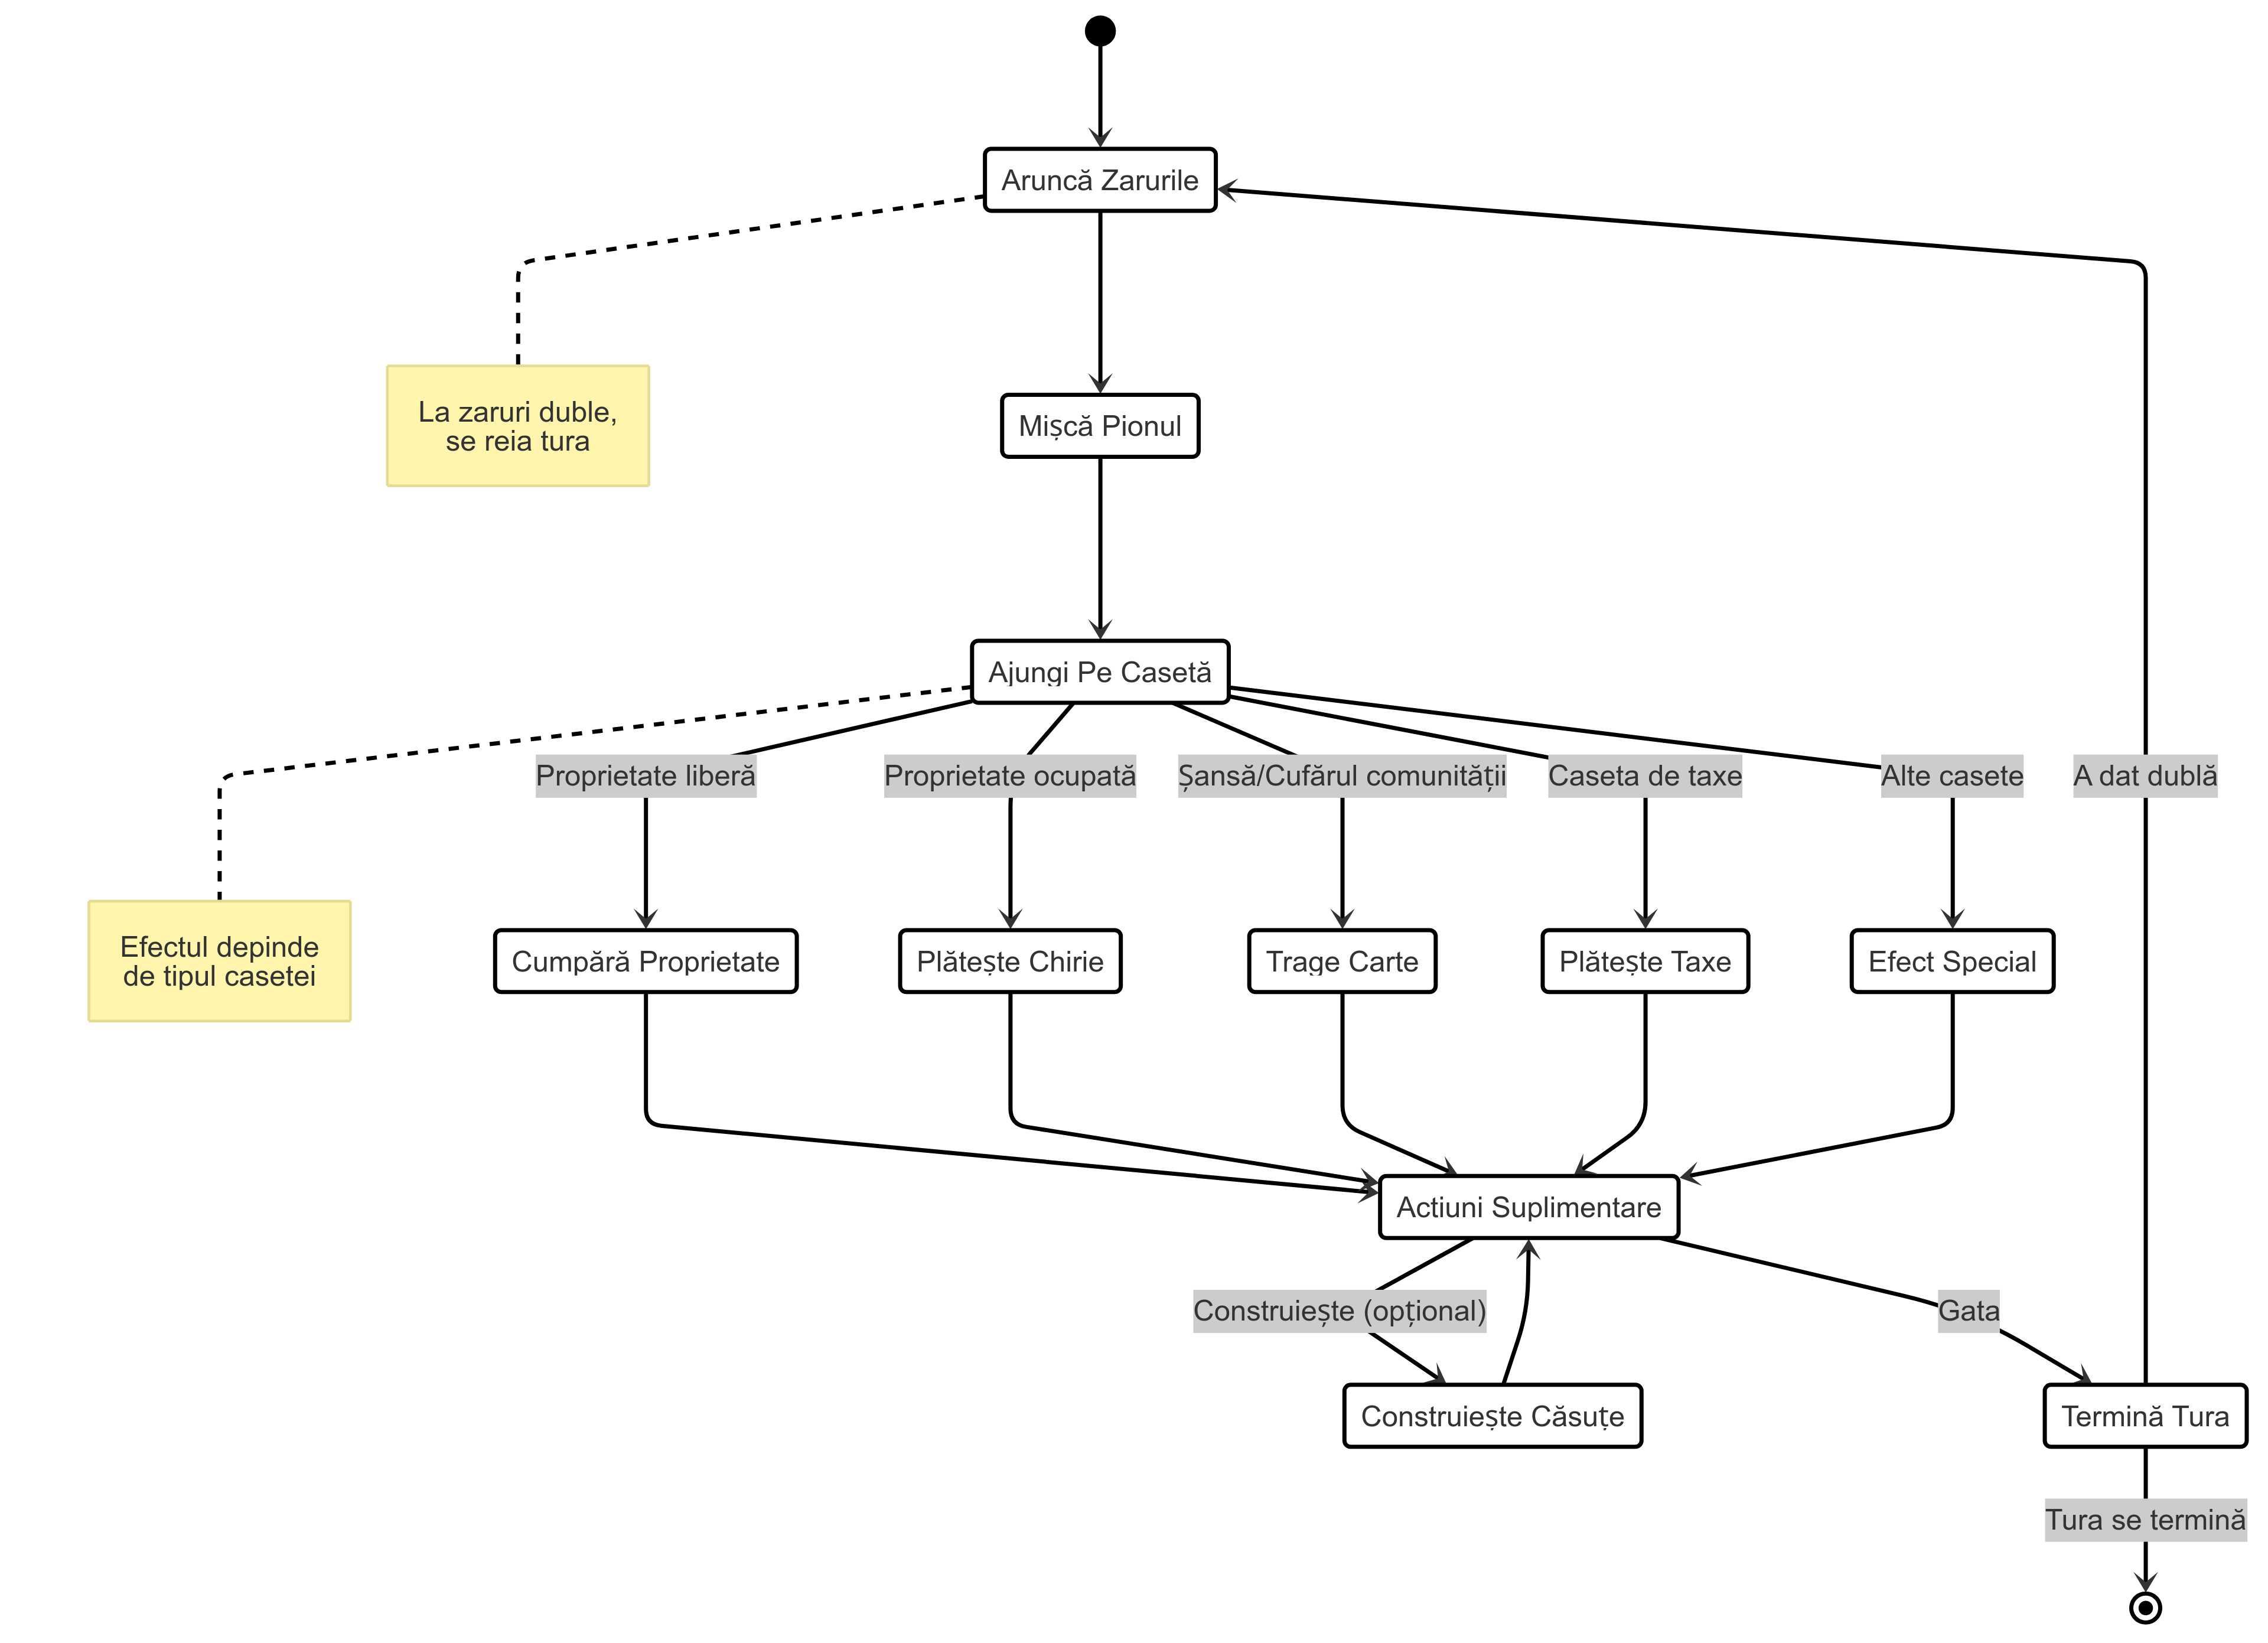
\includegraphics[width=10cm]{images/monopoly_rules_state_machine.png}
    \caption{Diagrama stărilor de joc și a acțiunilor posibile în Monopoly}
    \label{fig:monopoly-rules-state-machine}
\end{figure}

\subsection{Scopul jocului}
Fiecare jucător adună proprietăți, monopoluri, case și hoteluri de-a lungul unui episod. Scopul jocului este ca averea colectată din toate sursele, inclusiv banii cash, să fie cea mai mare. Decizia de încetare a jocului poate fi unanimă, moment în care fiecare jucător își calculează averea și se face poziționarea în clasament. Pe parcursul derulării jocului, dacă un jucător nu își poate plăti datoria, acesta este declarat falimentar și părăsește jocul. Ultimul jucător în joc este, de asemenea, considerat câștigător.

\section{Adaptări pentru reinforcement learning}
Datorită mediului digital și determinist ce constrânge implementarea realistă a jocului, câteva modificări vor trebui făcute pentru ușurarea atât a reprezentării cât și a redării fidele a unei reprize de joc.

Trebuie precizat că în ciuda intuiției naturale, anumiți factori de mediu pot influența dramatic buna desfășurare și simulare a jocului. Fiind un joc stocastic, bazat pe probabilitatea zarului, o statistică amănunțită \cite{monopoly_statistics} ne arată clar că nu toate proprietățile sunt uniform distribuite în cazul frecvenței vizitării lor. Acest lucru este de așteptat având în vedere distribuția probabilistică a zarurilor ce favorizează apariția numerelor 6, 7, 8 \cite{dice_statistics}.

Distribuția neuniformă poate influența și deciziile jucătorilor în estimarea venitului optim. Aceasta impune ca anumite proprietăți vor fi frecventate mai des decât altele \cite{monopoly_statistics_positions}, astfel impunându-se un factor bias în deciziile jucătorilor. Bazat pe frecvența vizitelor, se poate constata că o preponderență vizitare a culorii portocalii și a celei roșii ar aduce cel mai bun randament. Acest raționament se bazează pe ajungerea frecventă la închisoare, din multiple motive, iar distribuția neuniformă favorizând vizitarea căsuțelor corespunzătoare culorilor amintite, în urma ieșirii din închisoare.

Un alt lucru observabil este diminuarea realizărilor de monopoluri și uniformitatea jocului în cazul participării a mai mult de 2 jucători \cite{monopoly_statistic_players}. Nu doar că diferența de monopolizare crește, ba mai mult în cazul jocurilor cu mai mulți jucători, se observă clar o diferență în procentajul de câștig al jucătorilor care încep primii, aceasta putând ajunge și la 5\% diferență de procentaj în cazul ratei de câștig.

\subsection{Simplificarea regulilor}
Astfel observând regulile oficiale amintite anterior, dar și prin constatare personală în urma jucării Monopoly, am decis că anumite elemente sau aspecte pot fi reduse, fără a afecta negativ calitatea jocului sau influența rezultatul final.

O prima modificare va fi \textbf{limitarea numărului de jucători} la doar doi. Deși implementarea curentă poate susține un număr de până la 4 jucători, am decis că rezultatele și experimentele derulate să fie restrânse doar la doi jucători, pentru a favoriza dinamicitatea și posibilitatea dezvoltării rapide. Conform mențiunilor anterioare, un mediu cu prea mulți jucători se va baza exclusiv pe realizarea ofertelor de schimb pentru a se putea dezvolta monopoluri și a avea un rezultat final concludent. Mi-am dorit să elimin dependența de factori stocastici cât mai mult și să favorizez buna desfășurare a unui joc convergent către o stare definitivă. Astfel fiecare jucător va putea să își construiască și aplice strategia proprie fără a fi constrâns de factori externi.

O a doua modificare concludentă este \textbf{secvențierea acțiunilor} întreprinse. Dinamicitatea jocului ar fi îngreunat considerabil atât finalitatea unui episod, cât și reprezentarea sa eficientă. Un joc amical în lumea reală se bazează pe posibilitatea de interacțiune permanentă cu mediul chiar și în lipsa turului curent. Orice jucător poate, conform regulilor oficiale, să își îmbunătățească proprietățile, întreprindă schimburi, ipotecheze proprietăți, etc. în afara turului său. Decizia de urma modelarea conform standardelor actuale ar fi condus la o lipsă de convergență rapidă și o durată îndelungată a unui episod pentru a putea conchide asupra câștigătorului. Deși restricționează ferm acțiunile întreprinse, această modificare nu subvine în scopul schimbării interacțiunii, ci este doar o constrângere benefică în planificarea și consolidarea unui mecanism clar de acționare, defavorizând decizii spontane și adesea haotice. O bună detaliare asupra acestei secvențieri va fi detaliată în continuare.

Pe lângă modificările de mediu definitorii de mai sus, amintim și alte abăteri de la regulile oficiale cu scopul unei modelări mai agreabile ale environment-ului:
\begin{enumerate}
    \item \textbf{Procesul de licitație}: În regulile oficiale, în urma refuzului de achiziționare a unei proprietăți, aceasta trebuie supusă unei licitații, în care pot participa toți jucătorii, inclusiv cel care a refuzat. În urma unei analize, având la dispoziție doar doi jucători, procesul de cumpărare al unei proprietăți s-ar fi complicat linear, astfel am decis că achiziționarea unei proprietăți să fie o decizie binară cu putere de influențare nulă în exterior. Jucătorul care a ajuns pe proprietatea după mutare, poate fie să o cumpere, în cazul existenței fondurilor disponibile, fie să o refuze, astfel proprietatea rămânând în posesia băncii.
    \item \textbf{Dezvoltarea proprietăților}: Se face deodată, pentru întreg grupul de culoare, spre deosebire de regula standard, unde se poate face individual per proprietate. Această schimbare s-a făcut prin prisma constrângerii deciziei de investire cu planificare pe timp lung. Îmbunătățirea proprietăților ar trebui să fie o decizie importantă și un considerent major, nu doar o acțiune efectuată. Astfel prin această restrângere, fiecare jucător va trebui să cântărească atent decizia de a investi mai mulți bani deodată, cu promisiunea unui retur viitor al investițiilor.
    \item \textbf{Ignorarea limitelor resurselor}: Jocul oficial presupune existența unor resurse fizice limitate, precum bancnotele și casele/hotelurile. Am făcut abstracție de această limitare, dorind să ofer posibilitatea desfășurării strategiei optime. Într-adevăr, limitarea numărului de case și dispunerea acestora în urma unei licitații, ar fi crescut competitivitatea și previziunea jucătorilor, dar în același timp ar fi adăugat informație în plus de gestionat și îngreunat procesul simulării.
    \item \textbf{Dobânda proprietăților ipotecate}: Regulile curente ale jocului, privind plata unei dobânzi și ale unei sume adiționale în cazul ridicării ipotecii de pe o proprietate erau puțin complicate și de un interes scăzut. Astfel am decis că această regulă să fie ignorată și ridicarea ipotecii să poată fi făcută doar de jucătorul care a ipotecat-o, plătind cei 10\% din valoare proprietății.
    \item \textbf{Taxa pe venit}: Atunci când jucătorul ajunge pe căsuța "Taxa pe venit" are posibilitatea să plătească o sumă statică de 200₩ sau poate opta pentru plata a 10\% din totalul deținut, decizia trebuind luată fără a calcula cât reprezintă totalul deținut. Din cauza digitalizării jocului, această decizie ar fi fost trivială, totalul deținut fiind automat calculat și cunoscându-se de-a lungul jocului, fapt pentru care se va plăti constant suma de 200₩.
    \item \textbf{Sistemul de faliment}: Când un jucător nu își poate plăti o chirie, taxă sau orice sumă datorată, acesta este obligat să vândă ce are în scopul achitării datoriei, avand o singura sansa de redresare per actiune intreprinsa. În cazul în care nu reușește să strângă valoarea necesară, acesta este declarat "în faliment" (bankruptcy) și toată averea sa este împărțită în mod echitabil fiecărui jucător. În cazul nostru, având doar doi jucători, jocul se va termina iar jucătorul cu cea mai mare avere va fi declarat câștigător. De remarcat totuși, că implementarea oferă suport pentru a decide o alternativă a finalității jocului.
\end{enumerate}

\section{Arhitectura Generală a Sistemului}

\subsection{Principii de design}
În vederea construirii unui sistem reprezentativ, fidel și scalabil de simulare va trebui să avem în vedere separarea atribuțiilor și responsabilităților. Simulatorul nostru va trebui să mențină constant o stare a jocului cât mai fidelă de un joc real, asigurându-se constant că starea curentă și acțiunile efectuate respectă regulile impuse. De asemenea, acesta va trebui să permită adăugarea și modificarea jucătorilor folosind o metodă eficientă și va trebui să se asigure de coordonarea și secvențierea acțiunilor.

Mai mult de atât, va trebui să avem în vedere și nevoia simulării unui număr mare de jocuri, ceea ce ne constrânge să optimizăm sistemul și să ne asigurăm că acesta va funcționa fără probleme sub stres. Elementele sale trebuie să fie paralelizabile pentru a putea atât antrena cât și simula pe un număr cât mai mare de date într-un interval temporal predefinit.

\begin{figure}[H]
    \centering
    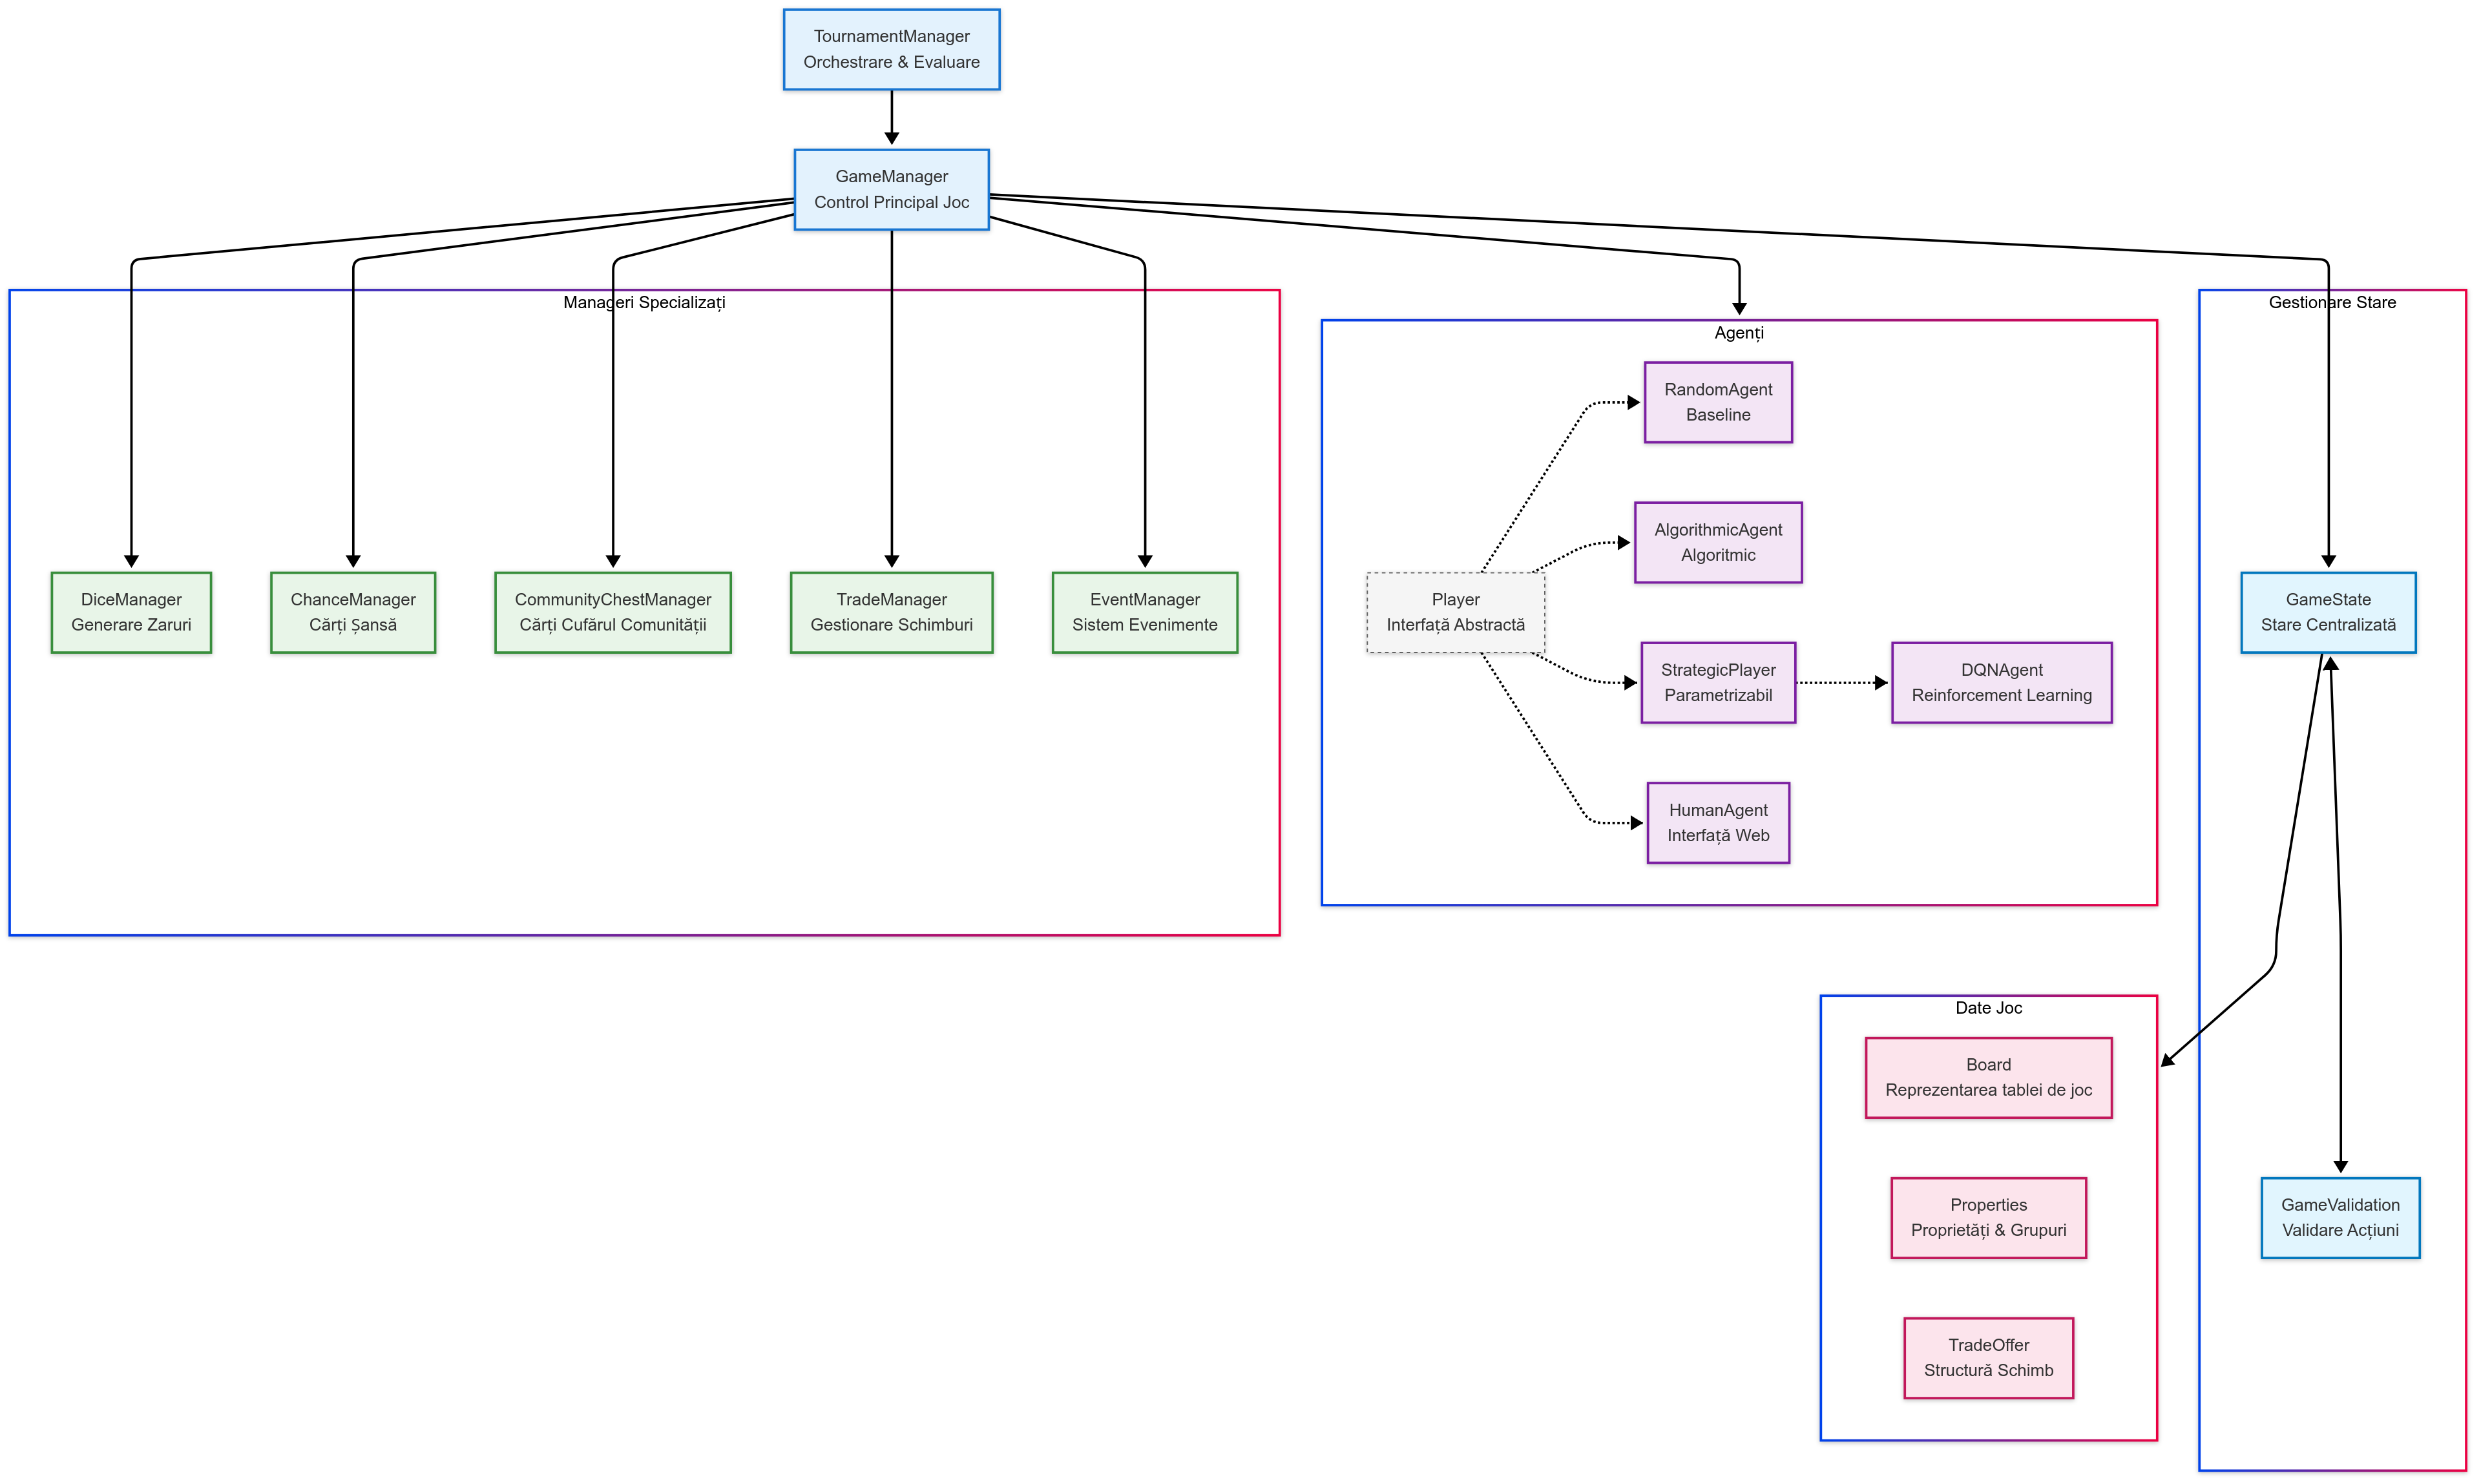
\includegraphics[width=15cm]{images/diagrama_flow.png}
    \caption{Diagrama arhitecturii generale a sistemului}
    \label{fig:diagrama-responsabilitati}
\end{figure}

\subsection{Separarea responsabilităților}
Delimitarea și îngrădirea răspunderii reprezintă un principiu de proiectare și arhitectură des întâlnit în lumea programării. Principiul responsabilității singulare (Principal of Singular Responsabilities) \cite{srp_desing_pattern}, face parte din familia principiilor SOLID \cite{solid_patterns} și favorizează scalabilitatea prin minimizarea funcționalităților unei entități. Minimizarea face ca testarea să fie mai unitară, iar dependințele mai puține, astfel crescând organizarea și lizibilitatea codului.

Menținerea principiului este evidențiată prin izolarea a trei componente importante în sistemul proiectat ce conlucrează împreună și se asigură de buna funcționare a simulării, conforme cu teorema:

\begin{displayquote}
\centering
\textit{Adună împreună lucrurile care se schimbă din aceleași motive. \\
Separă lucrurile care se schimbă din motive diferite.} \cite{srp_quote_source}
\end{displayquote}

Cele trei componente definitorii sunt:
\begin{itemize}
    \item \textbf{Sursa de adevăr}: Cea care se ocupă de menținerea constantă a reprezentării interne și fidele a jocului în orice moment de timp. Aceasta este singura ca poate modifica intern, în urma validărilor, starea jocului, la cerere din exterior și să se asigure că nu există probleme de integritate a datelor.
    \item \textbf{Orchestratorul central}: Cel care se ocupă de secvențierea acțiunilor, de derularea și simularea corectă a jocului, de interacțiunea dintre toate componentele, asigurând o bună funcționare a sistemului.
    \item \textbf{Jucătorii}: Cei care interacționează direct și produc schimbări în mediu, acționând voit printr-o politică internă cu scopul de a perturba și influența rezultatul jocului.
\end{itemize}

Pe lângă componentele principale enunțate anterior, se regăsesc și subcomponente ce preiau din atribuțiile părintelui și le segmentează în acțiuni atomice grupate. Acestea nu sunt decât niște extensii specializate, menite să ușureze și mai mult conceptualizarea reprezentării și ajutând cu evidențierea directă a nevoilor sistemului.

\subsection{Componentele sistemului}
Proiectarea arhitecturală anterioară ne oferă o bază bună de plecare în gândirea structurală a sistemului de simulare. Raportându-ne la aceasta putem implementa efectiv la nivel de cod toate noțiunile discutate anterior.

Datorită simplității, a folosirii sale pe scară largă, atât în domeniul cercetării, cât și în producerea de produse software, dar și a suportului vast, am preferat să folosesc ca și limbaj de programare Python \cite{python_org}. Acesta oferă suport pentru consolidarea structurilor și interacțiunilor prin clase, folosind paradigma de programare orientată pe obiecte \cite{geeksforgeeks_oops}.

În continuare vom reda principalele componente reprezentate sub forma de clase în codul nostru și vom explica importanța, responsabilitatea și câteva aspecte privind implementarea acolo unde cazul o va cere.

\subsubsection{Componentele de bază}
\subparagraph{GameState(starea jocului)}\label{game-state}
Reprezintă unica sursă de adevăr care încorporează toată informația regăsită într-un joc clasic de Monopoly, precum: poziția jucătorilor, jucătorul curent, banii fiecărui jucător, proprietățile deținute, etc. Acesta are la bază o subentitate a tablei de joc ce are ca scop oferirea informațiilor privind costul unei proprietăți, număr de entități dintr-o grupă de culoare, cât și alte informații utile în determinarea informațiilor privind tabla și cartonașele de joc.

Clasa este responsabilă de actualizarea atomică a fiecărei componente la cerere, prin intermediul unor metode predefinite. În caz de eroare, acesta o va propaga mai departe, neintrand în responsabilitatea sa tratarea erorilor.
\subparagraph{GameValidation(validarea jocului)}
O instanță de tip singleton \cite{geeksforgeeks_singleton} ce are drept scop asigurarea respectării integrării cu regulile jocului. Acesta expune metode de verificare ce semnalează prin returnarea unei erori, în cazul producerii uneia. Aici se definesc toate constrângerile necesare efectuării unei acțiuni.
\subparagraph{GameManager(coordonatorul jocului)}
Este orchestratorul principal asigurându-se că toate componentele principale și adiacente se comportă în modul așteptat. La bază acesta expune o metodă pentru simularea unui joc de Monopoly, pentru o stare de joc predefinită.

El creează succesiunea logică de acțiuni ce le întreprinde fiecare jucător la momentul rândului său, asigurându-se că jocul nu s-a terminat și nicio eroare nu a fost întâmpinată. Tratarea erorilor se va face din exterior, acesta doar propagându-le mai departe.

Gestionarea tuturor resurselor auxiliare, precum zarurilor, cartonașelor, etc., este făcută cu ajutor componentelor auxiliare. Acestea expun metode utilizate de clasa coordonatoare cu scopul determinării și întreprinderii acțiunii corespunzătoare.

O reprezentare detaliată a tranzițiilor în timpul unei ture a unui jucător va fi regăsită în anexă, aceasta necesând o explicație detaliată și o ilustrare complicată. Totuși, pentru o vizualizare rapidă și o înțelegere mai bună a modelării secvențiale a acțiunilor putem să observăm figura \ref{fig:monopoly-rules-state-machine}.

\subsubsection{Componentele auxiliare}
\subparagraph{DiceManager}
Se ocupă de generarea aleatoare a aruncărilor de zar, asigurându-se că aceasta se face cu o distribuție probabilistică uniformă. Pentru optimizare, din cauza numărului crescut de cerere, aruncările de zar sunt precalculate și stocate (cache-uite) pentru o și mai bună convergență și acuratețe privind probabilitatea.
\subparagraph{TradeManager}
Este actorul principal de întreprindere de schimburi, principala sa caracteristică fiind validarea și execuția schimburilor. Pentru că aceasta poate fi dinamică, atât din punct de vedere al numărului de oferte, cât și al obiectelor tranzacționate, acesta joacă un rol foarte important în asigurarea integrității și autenticității schimbului făcut.
\subparagraph{CommunityChestManager/ ChanceManager}
Sunt doi coordonatori ce împart responsabilitatea pentru categorii diferite de acțiuni, fiecare fiind reprezentativ pentru evenimentul stocastic de tragere a unui cartonaș "Cufărul Comunității", "Șansa" respectiv.

Acestea se asigură că există maxim două cărți de evadarea din pușcărie puse în circulație în același timp, și se ocupă de aranjarea și păstrarea ordinii cartonașelor de joc extrase. Ordinea de extragere și de plasare a cartonașelor respectă structura de coadă (queue) \cite{geeksforgeeks_queue} descrisă de regulile oficiale ale jocului. De asemenea sunt responsabili de definirea și executarea acțiunilor descrise pe cartonașele de joc.
\subparagraph{EventManager}\label{event-manager}
Entitatea de înregistrare și distribuire (broadcasting) ale evenimentelor reprezentative din joc. Acestea sunt înregistrate de alți manageri și partajate către toți jucătorii, prin intermediul unor metode expuse. Aceștia din urmă, jucătorii, pot decide în mod particular cum vor să trateze evenimentele și importanța alocată lor. Utilitatea acestei componente este evidențiată mai ales în folosirea ei în interfața grafică, fiind principala sursă de notificare.
\subparagraph{TournamentManager}\label{trade-manager}
O implementare personalizată a unui turneu între o listă de agenți predefiniți, ce captează informații de referință cu scopul unei analize detaliate asupra politicii și strategiilor aplicate. Acesta dispune și de opțiunea de duel în stilul round-robin \cite{wikipedia_roundrobin}, având numeroare optimizări de paralelizare și multiprocesare pentru accelerarea vitizei de calcul.

\subsubsection{Arhitectura agenților}

\begin{figure}[h]
    \centering
    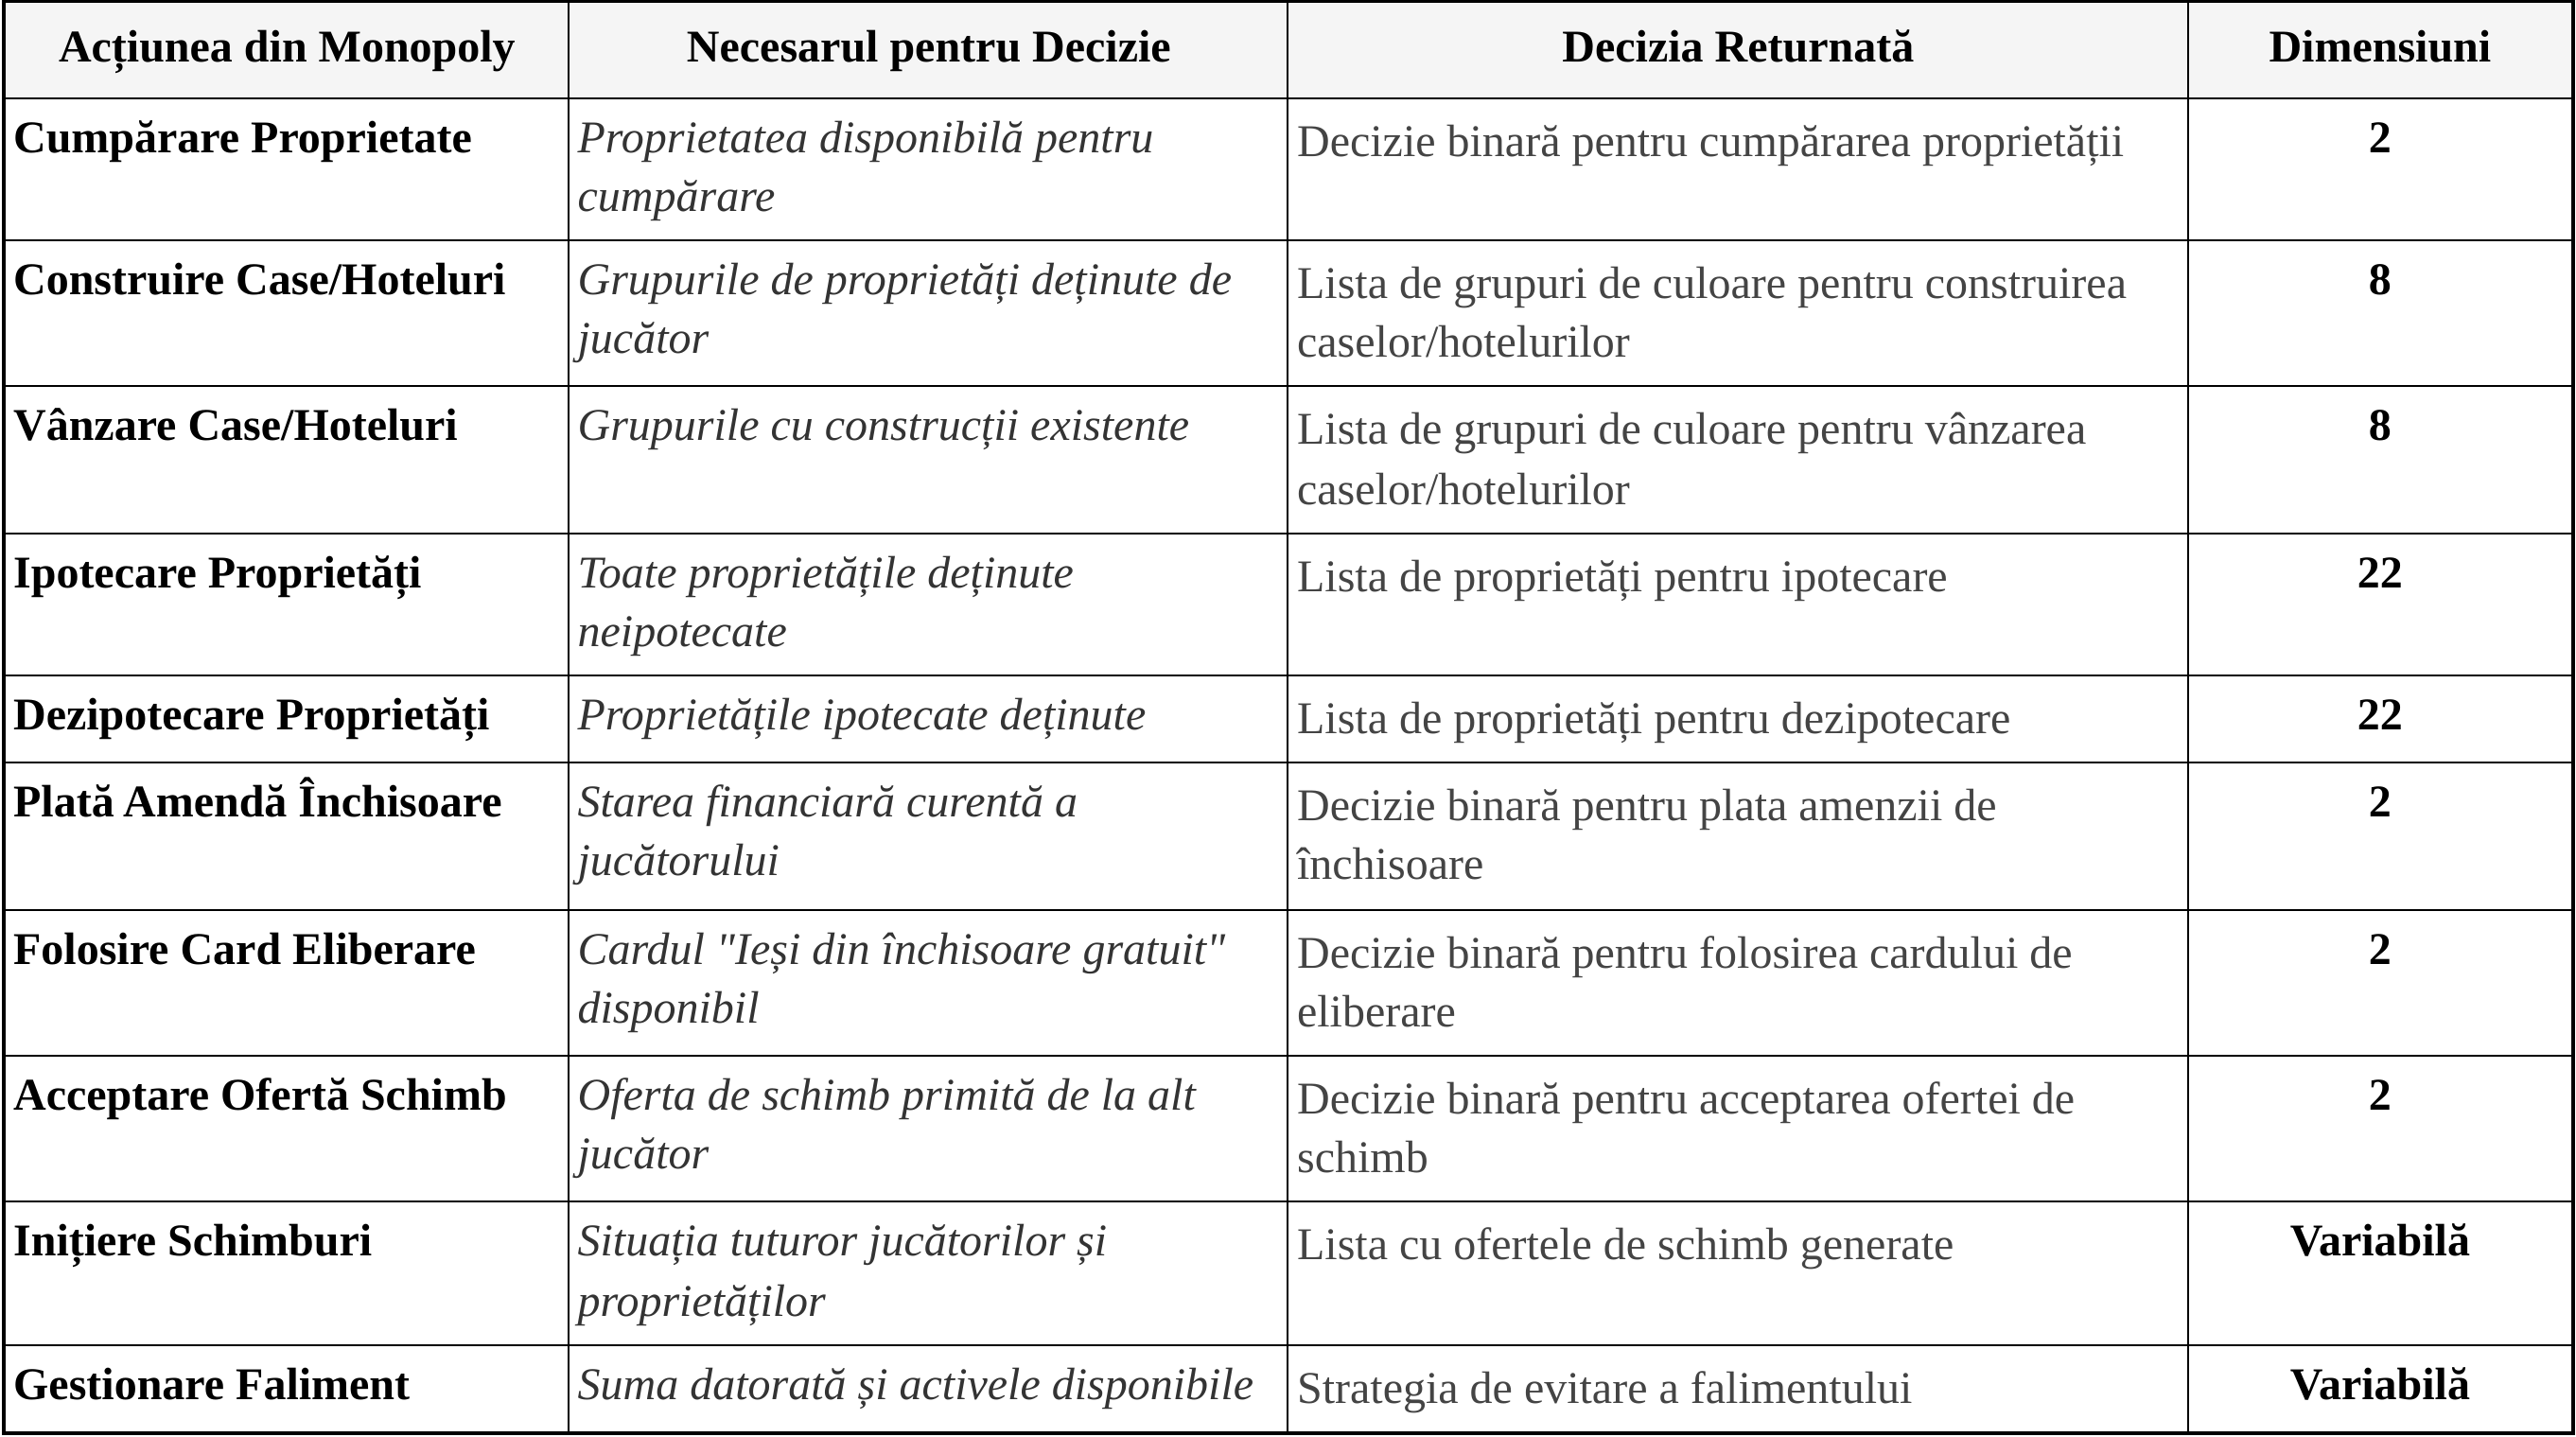
\includegraphics[width=16cm]{images/monopoly_actions_html_table (1).png}
    \caption{Actiunile permise in simulatorul de Monopoly}
    \label{fig:monopoly_actions}
\end{figure}

\subparagraph{Player}
Interfața Player (Jucător) este clasa de bază pentru definirea unui jucător care să interacționeze cu mediul creat. Aceasta asigură metodele de bază pentru definirea modului de interacțiune, așa cum este redat în tabelul \ref{fig:monopoly_actions}. Orice instanță de jucător dezvoltată ulterior, va trebui să moștenească din această clasă și să își suprascrie metodele prezentate anterior.

De asemenea, clasa părinte oferă și o implementare de bază a funcției de receptare și prelucrare a evenimentelor primite, pentru ușurarea codului și simplitate. Jucătorii care vor moșteni interfața Player vor fi numiți generic agenți, din terminologia specifică învățării prin întărire \cite{geeksforgeeks_marl}.

\subparagraph{Agentul Random}
Este un agent care execută orice acțiune într-o manieră stocastică, fără a avea vreo bază algoritmică sau politică predefinită. Este folosit ca și referință de bază în evaluarea celorlalți agenți. Acesta poate găsi din întâmplare un parcurs bun în cadrul unui episod, nimerind o politică optimă.

\subparagraph{Agentul Algoritmic}
Este o implementare simplistă de abordare algoritmică, ce își bazează raționamentele pe calcule simple și observări superficiale ale mediului. Acesta servește ca și punct de referință în cadrul raportării și descrierii unui comportament inteligent.

\subparagraph{Agentul Strategic Configurabil}
Este un superset, total îmbunătățit al abordării algoritmice, ce are în vedere o politică evoluată de observare și abordare a mediului. Acesta își bazează acțiunile pe multiple evaluări și o previziune de durată a costului efectuării unei acțiuni.

De asemenea, este construit să fie parametrizabil prin 28 de parametri ce deservesc ca pivoți în deciziile efectuate. Alături de configurarea standard, am studiat alte 9 configurări ale acestuia utilizând diferite scenarii.

\subparagraph{Agentul Uman}
Este o interfață grafică de utilizare și testare a celorlalți agenți, fiind construită ca punct de observație și dovedire practică a capacităților de învățare ale agentului inteligent. Acesta folosește ca și mediu browser-ul web, având construit în spate (backend) un server în Python.

\subparagraph{Agentul DQN}
Agentul inteligent, bazat pe învățare prin întărire, având numeroase rețele neuronale și fiind antrenat pe mai multe milioane de experiențe, reprezintă obiectivul tezei curente. Acesta își bazează acțiunile pe experiența dobândită și pe corelațiile pe care a reușit să le deprindă în timpul antrenamentului.